%*******************************************************************************
%*********************************** First Chapter *****************************
%*******************************************************************************

\chapter{Posture Generation, state of the Art, Introduction}


\nomenclature[z-PG]{PG}{Posture Generation}
\nomenclature[z-IK]{IK}{Inverse Kinematics}
\nomenclature[z-dof]{dof}{degrees of freedom}


\graphicspath{{Chapter1/Figs/Vector/}{Chapter1/Figs/}}

\section{List of contributions}
\begin{itemize}
  \item Generalities, introduction
  \item Presentation of the existing methods
  \item From Inverse Kinematics to Generalized IK/posture Generation/pose estimation (addition of articular limits, forces, stability etc.
  \item Topology of the parametrization space (Free-flyer, q, f, other)
  \item Formulation as a non-linear constrained optimization problem
  \item Adrien \& Karim's formulations
  \item Formulation of several types of cost/constraints
  \begin{itemize}
    \item Contact with plane surface
    \item Collision avoidance
    \item Auto-Collision avoidance
    \item Static equilibrium: Newton/CoM projection
    \item Forces in friction cones
    \item Articular limits
    \item Torque limits
    \item Torque minimization
    \item Goal Posture
  \end{itemize}
  \item Reasons why it is not enough and why we needed a new PG
    \begin{itemize}
      \item Having an easier way to formulate problems
      \item Avoid having to de some gymnastic to remain on manifolds
      \item Automatic variable management
      \item Robustness
    \end{itemize}
  \item Utilization of posture generation in planning
\end{itemize}


%%%%%%%%%%%%%%%%%%%%%%%%%%
%  SECTION INTRODUCTION  %
%%%%%%%%%%%%%%%%%%%%%%%%%%

\section{Introduction}
\label{sec:introduction}



The ultimate goal of robotics is to make robots realize some tasks.
The tasks, as well as the robot used to fulfill are various.
For example, it can be a robotic arm building a car in a factory, a surgeon robot operating on a human, a submarine robot exploring the wreckages of a ship, a humanoid robot exploring and fixing a destroyed nuclear plant.
\begin{figure}[ht]
  \centering
  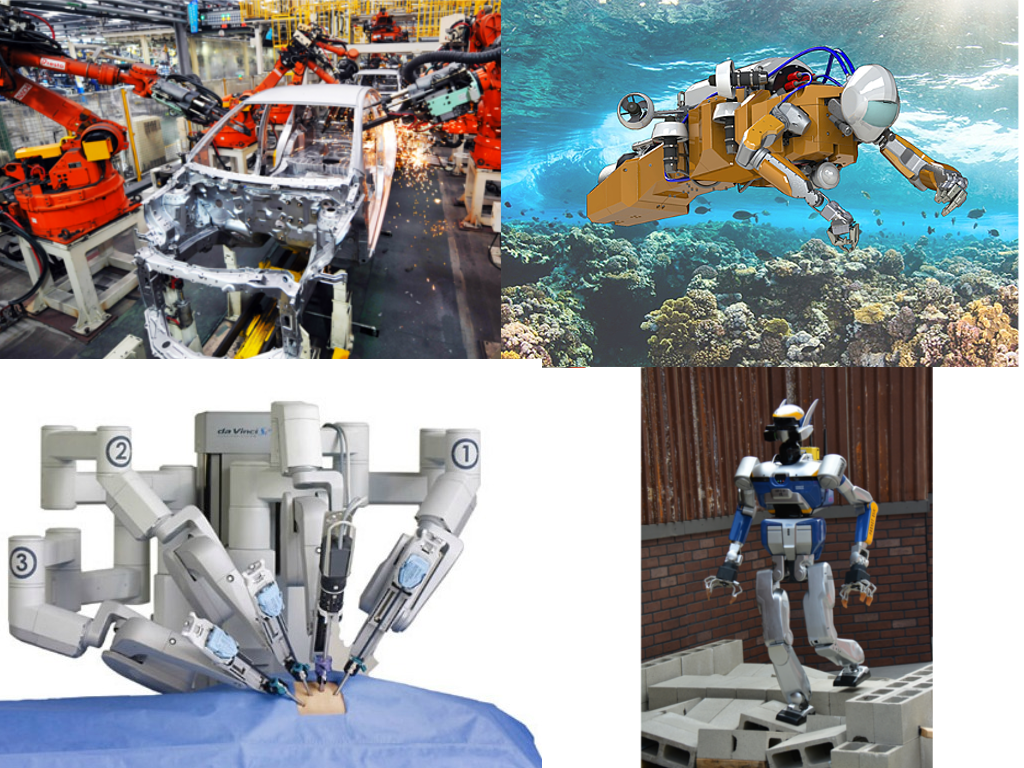
\includegraphics[width=0.9\textwidth]{various-tasks.png}
  \caption{Various robots doing various tasks}
  \label{fig:various}
\end{figure}

The DARPA Robotics Challenge has brought some light on the humanoid robots.
This competition brought together a large scope of robotics groups from universities, laboratories and private companies around a common goal: Make a robot succeed in several challenges without any human physical intervention.
The robots were expected to drive a car, open a door, climb stairs, cross debris, drill a hole in a wall, etc.
All those tasks can usually be broken down into sets of elementary tasks in human language.
Some typical examples of tasks for a robot can be "Put hand in contact with target", "Put foot on next step", "Avoid collision with that object", "Maintain stability" or "Look in that direction".
As is, those tasks do not mean anything for the robot.
A robot is made of a collection of bodies that are linked together by joints, that are actuated by motors.
A robots configuration consists of the position and orientation of the robot's base body, a vector of joint parameter defining the configuration of each joint of the robot and a vector of joint efforts defining the efforts exerted by actuators in each joint.
Satisfying a task requires to control the joints of the robot so that the whole system reaches a configuration that satisfies the task.
The action of satisfying a task comes down to moving from an initial configuration to a goal configuration, figuring out the trajectory to follow and actually following it are the jobs of the trajectory generation and the control of the robot.
Those are by themselves some complete fields of robotics, and they have one thing in common, they both need to be given an initial configuration, a final configuration and sometime some intermediate configurations.
Finding those configurations is the job of what we call the Posture Generation (PG), which is the main topic of this dissertation.

\section{Problem Definition}
\label{sec:problem_definition}

We consider a robot $\mathit{R}$ with $n$ degrees of freedom (dof), its joint configuration can be described by a point on

\section{From Inverse Kinematics to Posture Generation}
\label{sec:from_inverse_kinematics_to_posture_generation}

The problem of finding a configuration of a polyarticulated system to satisfy some geometric constraints has been widely studied for decades under the name of Inverse Kinematics (IK).
IK is an important tool in many fields like robotics, computer graphics and animation.




%%%%%%%%%%%%%%%%%%%%%%%%%
%  SECTION FORMULATION  %
%%%%%%%%%%%%%%%%%%%%%%%%%

\section{Formulation}

Here we present the basic formulation of a PG problem.

The free-flyer, the articular space and the forces being the usual variables.

Presentation of all the constraints and their formulation
\begin{itemize}
  \item Joint limits
  \item Auto-collision
  \item Collisions with environment
  \item Contacts with environment
  \item Stability
  \item Torque limits
\end{itemize}

